% concatenated from main.tex
\documentclass[11pt]{article}
\usepackage{amsmath,amsthm}
\usepackage{amssymb}
\usepackage{bm}
\usepackage{subcaption}
\captionsetup{subrefformat=parens,font=small}
\usepackage{xcolor}
\usepackage{tikz}
\usetikzlibrary{calc}

\usepackage{geometry}
\geometry{left=28mm,right=28mm,
top=26mm,bottom=26mm}

\usepackage[colorlinks=true,
linkcolor=blue,citecolor=blue,
urlcolor=blue,pagebackref]{hyperref}

\makeatletter
\def\@seccntDot{.}
\def\@seccntformat#1{\csname the#1\endcsname\@seccntDot\hskip 0.5em}
\renewcommand\section{\@startsection{section}{1}{\z@}%
{18\p@ \@plus 6\p@ \@minus 3\p@}%
{9\p@ \@plus 6\p@ \@minus 3\p@}%
{\large\bfseries\boldmath}}
\renewcommand\subsection{\@startsection{subsection}{2}{\z@}%
{15\p@ \@plus 6\p@ \@minus 3\p@}%
{6\p@ \@plus 6\p@ \@minus 3\p@}%
{\itshape}}
\renewcommand\subsubsection{\@startsection{subsubsection}{3}{\z@}%
{12\p@ \@plus 6\p@ \@minus 3\p@}%
{\p@}%
{}}
\makeatother

\usepackage{microtype}
% \usepackage{showkeys}

%%%%%%%%%%%%%%%%%%%%%%%%% Setting of Theorem Style %%%%%%%%%%%%%%%%%

\theoremstyle{plain}
\newtheorem{theorem}{Theorem}[section]
\newtheorem{lemma}{Lemma}[section]
\newtheorem{corollary}{Corollary}[section]
\newtheorem{proposition}{Proposition}[section]
\newtheorem{problem}{Problem}[section]
\newtheorem{conjecture}{Conjecture}[section]

\theoremstyle{definition}
\newtheorem{definition}{Definition}[section]
\newtheorem{remark}{Remark}[section]
\newtheorem{example}{Example}[section]
\newtheorem{claim}{Claim}[section]

%%%%%%%%%%%%%%%%%%%%%%%%%%%%%%%%%%%%%%%%%%%%%%%%%%%%%%%%%%%%%%%%%%

\numberwithin{equation}{section}
\allowdisplaybreaks
\parindent=18pt
\renewcommand{\baselinestretch}{1.1}

\title{A complete solution to the Boots-Royle/Cao-Vince conjecture}
 

% \title{A complete solution to a conjecture on the extremal spectral radius of planar graphs}

\author{Lele Liu\footnote{School of Mathematical Sciences, Anhui University, Hefei 230601,
P.R. China. E-mail: \texttt{liu@ahu.edu.cn} (L. Liu). Supported by the National
Nature Science Foundation of China (No. 12471320), and Anhui Provincial Natural Science Foundation for Excellent Young Scholars (No. 2408085Y003).}\,~~~~
Bo Ning\footnote{College of Cryptology and Cyber Science \& College of Computer Science, Nankai University, Tianjin 300350, P.R. China.
E-mail: \texttt{bo.ning@nankai.edu.cn} (B. Ning). Partially supported by the National Nature Science
Foundation of China (No. 12371350) and Fundamental Research Funds for the Central Universities, Nankai University (No. 63243151).}\,~~~~
Yi Wang\footnote{School of Mathematical Sciences, Anhui University, Hefei 230601,
P.R. China. E-mail: \texttt{wangy@ahu.edu.cn} (Y. Wang).
Supported by the National Natural Science Foundation of China (No. 12171002, 12331012)}
}

\date{}


\begin{document}
\maketitle

\begin{abstract}
Boots and Royle, and independently Cao and Vince, conjectured that the join of an edge and a path 
on $n-2$ vertices is the unique planar graph of maximum adjacency spectral radius for $n\geq 9$. 
Tait and Tobin (JCTB, 2017) proved the conjecture for sufficiently large order. In this paper, 
we completely resolved the Boots-Royle/Cao-Vince conjecture.
\par\vspace{2mm}
\noindent{\bfseries Keywords:} Spectral radius; Planar graph; Perron vector; Spectral extremal graph theory.
\par\vspace{2mm}
\noindent{\bfseries AMS Classification:} 05C35; 05C50; 15A18
\end{abstract}



\section{Introduction}
Let $G$ be a simple graph, and let $\lambda(G)$ denote the spectral radius of its
adjacency matrix. A classical problem at the intersection of spectral graph
theory and topological graph theory is to determine how large $\lambda(G)$ can be
when $G$ is planar, and, more ambitiously, to characterize all graphs attaining
the maximum. The study of this problem goes back at least to Schwenk and
Wilson~\cite{SchwenkWilson1978}. In 1988, Hong \cite{Hong1988} proved that every planar
graph of order $n$ satisfies $\lambda(G)\leq \sqrt{5n-11}$ by using the famous Hong's spectral 
inequality and Euler formula. Cao and Vince~\cite{CaoVince1993} subsequently improved this
estimate to $\lambda(G) < 4 + \sqrt{3n-9}$. Further improvements were obtained by 
Hong~\cite{Hong1995,Hong1998}, and Ellingham and Zha~\cite{EllinghamZha2000} later established the bound
$\lambda(G)\leq 2+\sqrt{2n-6}$. These results progressively narrowed the gap between the known upper bounds
and the natural planar constructions $K_2\vee P_{n-2}$, where $\vee$ denotes the graph join. They also shifted attention from merely
estimating the spectral radius to the more delicate problem of determining the exact extremal graph.

There are two famous conjectures in the related area. The first concerns outerplanar graphs. 
In their 1990 survey \cite{CvetkovicRowlinson1990}, Cvetkovi\'c and Rowlinson conjectured
that $K_1\vee P_{n-1}$ attains the maximum spectral radius among all outerplanar graphs of order $n$. Following partial results of Rowlinson,
Cao and Vince \cite{CaoVince1993}, Tait and Tobin~\cite{TaitTobin2017} confirmed the
conjecture for all sufficiently large $n$. The remaining finite part was
eventually settled by Lin and Ning~\cite{LinNing2021}, who proved that the
conjectured fan is extremal for every $n\geq 2$, with $n=6$ as the unique
exception. The proof is with aid of a result of Shu and Hong \cite{ShuHong2000}, which states that $\lambda(G)\leq 3/2 + \sqrt{n - 7/4}$.
Thus, the outerplanar spectral extremal problem is now completely
understood.

The second and more difficult conjecture is about planar graphs. Motivated in part by the use 
of the spectral radius as a measure of the connectivity of planar networks, Boots and Royle~\cite{BootsRoyle1991}
conjectured in 1991 that, for every $n\geq 9$, the unique planar graph of order
$n$ with maximum spectral radius is $K_2\vee P_{n-2}$. The same conjecture was proposed independently 
by Cao and Vince~\cite{CaoVince1993}. 

\begin{conjecture}[Boots-Royle-Cao-Vince]
Among all planar graphs on $n\geq 9$ vertices, $K_2\vee P_{n-2}$ attains the maximum spectral radius.   
\end{conjecture}

\begin{figure}[htbp]
\centering
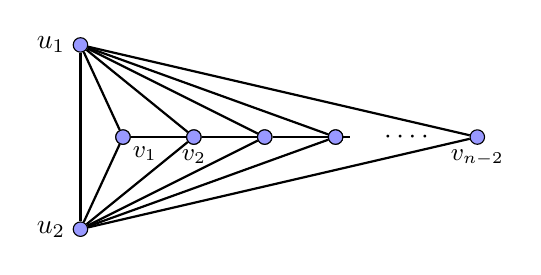
\begin{tikzpicture}[main_node/.style={circle,draw,fill=blue!40,inner sep=.65mm}, scale=.9]
\node[main_node] (u1) at (-0.6, 1.3) {};
\node[main_node] (u2) at (-0.6, -1.3) {};
\node[main_node] (v4) at (5, 0) {};

\foreach \i in {0,1,...,3}
{%
\node[main_node] (v\i) at (\i, 0) {};
\draw[thick] (u1) -- (v\i);
\draw[thick] (u2) -- (v\i);
}

\draw[thick][thick] (v0) -- (v1) -- (v2) -- (v3);
\draw[thick] (u1) -- (u2);
\draw[thick] (u1) -- (v4) -- (u2);
\draw[thick] (v3) -- (3.2,0);
\node at (4,0) {$\cdots\cdot$};

\foreach \i in {0,1,...,3}
{%
\node[main_node] (v\i) at (\i, 0) {};
}

\node[left=2pt] at (u1) {$u_1$};
\node[left=2pt] at (u2) {$u_2$};
\node[anchor=north west] at (v0) {\small $v_1$};
\node[below=1pt] at (v1) {\small $v_2$};
\node[below=1pt] at (v4) {\small $v_{n-2}$};
\end{tikzpicture}
\caption{The graph $K_2\vee P_{n-2}$}
\label{fig:candidate}
\end{figure}

An important improvement was announced in Guiduli's 1996 doctoral dissertation \emph{Spectral Extrema for Graphs}
at the University of Chicago, written under the supervision of Babai~\cite{Guiduli1996}. It was later reported 
that Guiduli and Hayes had proved, in an unpublished preprint, that the planar conjecture holds for
sufficiently large $n$; however, that manuscript never appeared in published form (see also the introduction 
of Tait and Tobin \cite{TaitTobin2017}). In 2017, Tait and Tobin~\cite{TaitTobin2017} proved
that $K_2\vee P_{n-2}$ is indeed the unique planar graph of maximum spectral radius whenever $n$ is sufficiently large.

The original conjecture was formulated for $n\geq 9$. The purpose of this paper is to give a complete proof of the conjecture. 

\begin{theorem}\label{thm:main}
For every $n\geq 3$, except for $n\in\{7,8\}$, the graph $K_2\vee P_{n-2}$ is the unique 
planar graph on $n$ vertices with maximum adjacency spectral radius. For $n\in\{7,8\}$, 
the extremal graphs are the exceptional graphs shown in Figure~\ref{fig:extremal-graphs-7-8}.
\end{theorem}

\begin{figure}[htbp]
\centering
\subcaptionbox{$n=7$ \label{subfig:7-vertex}}[.44\textwidth]{%
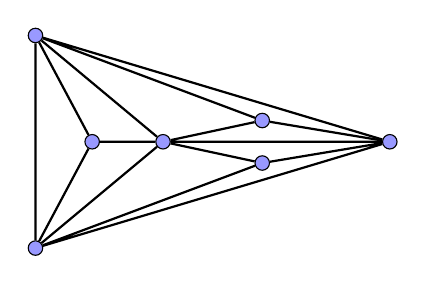
\begin{tikzpicture}[main_node/.style={circle,draw,fill=blue!40,inner sep=.65mm}, scale=.9]

\node[main_node] (0) at (1.8, 0) {};
\node[main_node] (1) at (5, 0) {};
\node[main_node] (2) at (3.2, -.3) {};
\node[main_node] (3) at (0, -1.5) {};
\node[main_node] (4) at (0.8, 0) {};
\node[main_node] (5) at (0, 1.5) {};
\node[main_node] (6) at (3.2, .3) {};

\draw[thick] (5) -- (0) -- (1) -- (2) -- (3) -- (4) -- (5) -- (6) -- (0) -- (3) -- (5) -- (1) -- (3);
\draw[thick] (2) -- (0) -- (4); 
\draw[thick] (1) -- (6); 
\end{tikzpicture}
}
\subcaptionbox{$n=8$ \label{subfig:8-vertex}}[.44\textwidth]{%
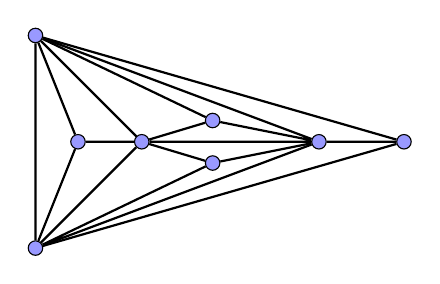
\begin{tikzpicture}[main_node/.style={circle,draw,fill=blue!40,inner sep=.65mm}, scale=.9]

\node[main_node] (0) at (0, -1.5) {};
\node[main_node] (1) at (0, 1.5) {};
\node[main_node] (2) at (.6, 0) {};
\node[main_node] (3) at (1.5, 0) {};
\node[main_node] (4) at (2.5, -.3) {};
\node[main_node] (5) at (4, 0) {};
\node[main_node] (6) at (5.2, 0) {};
\node[main_node] (7) at (2.5, .3) {};

\draw[thick] (0) -- (1) -- (2) -- (3) -- (4) -- (5) -- (6) -- (0) -- (2);
\draw[thick] (0) -- (3) -- (1) -- (5) -- (3) -- (7) -- (5) -- (0) -- (4);
\draw[thick] (6) -- (1) -- (7);
\end{tikzpicture}
}
\caption{The planar graphs with maximum spectral radius for $n=7,8$}
\label{fig:extremal-graphs-7-8}
\end{figure}

The corresponding problem for graphs embeddable on surfaces of arbitrary genus provides a broader 
setting for these results. Let $\operatorname{spex}(n,\gamma)$ denote the maximum spectral radius of an
$n$-vertex graph embeddable on a surface of Euler genus $\gamma$. Hong
initiated its systematic study and obtained, among other genus-dependent bounds,
$\operatorname{spex}(n,\gamma) \leq 1+\sqrt{3n+6\gamma-8}$. Ellingham and Zha \cite{EllinghamZha2000} improved this to $2+\sqrt{2n+8\gamma-6}$. Very recently, 
Zhai, Fang and Lin~\cite{ZhaiFangLin2026} proved that, for each fixed $\gamma$ and all
sufficiently large $n$, every spectral-extremal graph is obtained from $K_2\vee P_{n-2}$ by 
adding exactly $3\gamma$ edges inside a bounded core. Related extremal questions have also 
been studied for the tensor spectral radius of uniform hypergraphs. In particular, Ellingham, Lu and Wang~\cite{EllinghamLuWang2022} established an outerplanar $3$-uniform hypergraph analogue of 
the Cvetkovi\'c--Rowlinson conjecture for all sufficiently large orders.

We conclude this section with an outline of the paper. In Section \ref{sec:notation}, we
introduce the notation and preliminary tools, including a lower bound on the extremal spectral radius
supplied by $K_2\vee P_{n-2}$. Section \ref{sec:series-lemmas} focuses on cubic vertices in
an extremal plane triangulation, deriving constraints on the three largest Perron entries that lead to the structural inequalities essential for the subsequent arguments. In
Section \ref{sec:first-universal-vertex}, we prove that every extremal graph must contain a vertex of degree $n-1$. Section \ref{sec:second-universal-vertex} applies a similar analysis to that of Section \ref{sec:series-lemmas}, now in the setting of outerplanar graphs, to force the existence of a second universal vertex. Finally, Section \ref{sec:finish-proof}
uses the two universal vertices and planarity to identify the remaining graph
as a path, which completes the proof.


\section{Notation and preliminary results}
\label{sec:notation}

For a graph $G$ on $n$ vertices, we write $e(G)$ for the number of edges of $G$. For a vertex $v$, 
we write $N_G(v)$ and $N_G[v]$ for its open and closed neighborhoods, respectively, 
and $d_G(v)$ for its degree. In the above notation, we will skip the subscript $G$ 
when $G$ is clear from context. 
We refer to a vertex of degree $3$ as a \emph{cubic vertex}; and a vertex of degree $n-1$ as a \emph{universal vertex}.
We also use the usual facts about plane triangulations and maximal outerplanar graphs; 
see, for example, \cite[Chapter 10]{BondyMurty}.

\begin{theorem}[Liu--Weng \cite{LiuWeng}]\label{thm:degree}
Let $G$ be a connected graph on $n$ vertices with degree sequence
$d_1\geq d_2\geq\cdots\geq d_n$. For every $1\leq j\leq n$,
\[
\lambda(G)\leq \frac{d_j - 1 + \sqrt{(d_j+1)^2 + 4\sum_{i=1}^{j-1} (d_i - d_j)}}{2}.
\]
\end{theorem}

The following lemma is a consequence of Cauchy interlacing theorem, also known as the Poincar\'e 
Separation Theorem (see, e.g., \cite{Haemers1995} or \cite[Corollary 4.3.37]{Horn-Johnson2012}).

\begin{lemma}[\cite{Haemers1995} or {\cite[Corollary 4.3.37]{Horn-Johnson2012}}]\label{lem:interlace-inequality}
Let $S$ be a real $n\times m$ matrix such that $S^{\mathrm{T}} S = I$ and let $A$ be a 
symmetric $n\times n$ matrix with eigenvalues $\lambda_1\geq\cdots\geq\lambda_n$. Define $B = S^{\mathrm{T}} AS$ 
and let $B$ have eigenvalues $\mu_1\geq\cdots\geq\mu_m$. Then 
\[
\mu_i(B) \leq\lambda_i(A)\leq\mu_{i+n-m}(B), \quad i=1,2,\ldots,m.
\]
\end{lemma}

We next derive a lower bound on $\lambda(K_2\vee P_{n-2})$. Put
\[
 H_n:= K_2\vee P_{n-2}, \qquad r_n:= \frac{3 + \sqrt{8n-19}}{2}.
\]

\begin{lemma}\label{lem:benchmark}
For every $n\geq 10$, $\lambda (H_n) > r_n$.
\end{lemma}

\begin{proof}
Let the two universal vertices of $H_n$ be $u_1,u_2$, and let $v_1,v_2,\ldots,v_{n-2}$ 
be the path in its natural order (see Fig. \ref{fig:candidate}).  
Put $q=n-4$. Consider the three orthonormal vectors
\[
 f_1 = \frac{\bm{e}_{u_1} + \bm{e}_{u_2}}{\sqrt{2}}, \qquad
 f_2 = \frac{\bm{e}_{v_1} + \bm{e}_{v_{n-2}}}{\sqrt{2}}, \qquad
 f_3 = \frac{1}{\sqrt{q}} \sum_{i=2}^{n-3} \bm{e}_{v_i}.
\]
If $S=(f_1\ f_2\ f_3)$, then $S^{\mathrm{T}} S = I_3$. A direct computation of $Q_n = S^{\mathrm{T}} A(H_n) S$ yields
\[
Q_n =
\begin{bmatrix}
 1 & 2 & \sqrt{2q} \\
 2 & 0 & \sqrt{2/q} \\
 \sqrt{2q} & \sqrt{2/q} & 2(q-1)/q
\end{bmatrix}.
\]
By Lemma \ref{lem:interlace-inequality}, we find
$\lambda(H_n)\geq\rho(Q_n)$, where $\rho(Q_n)$ is the largest eigenvalue of $Q_n$.

Since $\mathrm{tr} (Q_n) > 0$, $Q_n$ has at least one positive eigenvalue. 
Also, the $2$-th leading principal minors of $Q_n$ is negative, we know $Q_n$
has at least one negative eigenvalue. Since the product of all three eigenvalues is positive, 
$Q_n$ has exactly one positive eigenvalue.

Expanding the determinant of $r_n I - Q_n$, and using the identity $r_n^2 - 3r_n = 2n-7=2q+1$, gives
\begin{align*}
q\cdot\det(r_nI - Q_n)
& = qr_n(r_n - 1)(r_n - 2) - 4qr_n - 2q^2 r_n + 2(r_n - 1)^2 - 8 \\
& = 4q - 4 - r_n(q - 2).
\end{align*}
Consequently, $\det (r_nI - Q_n) < 0$. 

The two negative eigenvalues of $Q_n$ contribute positive factors to
$\det(r_nI - Q_n)$. Hence $\det (r_nI - Q_n) < 0$ forces the unique positive eigenvalue of $Q_n$ to be
larger than $r_n$. Combining this with $\lambda(H_n) > \rho(Q_n)$ proves $\lambda(H_n) > r_n$.
\end{proof}

\section{Cubic vertices in an extremal triangulation}
\label{sec:series-lemmas}

Throughout the remainder of the paper, let $G$ be a planar graph of order $n\geq 15$ having 
maximum spectral radius, and put $\lambda := \lambda(G)$. Let $\bm{x} = (x_v)_{v\in V(G)}$ 
be a nonnegative Perron vector, normalized by $\|\bm{x}\|_1 = 1$. Since $H_n$ is planar, extremality and Lemma~\ref{lem:benchmark} imply $\lambda > r_n$.

Two consequences of $G$ being planar that we will use frequently are that $G$ has at most $3n-6$ edges and $G$ does not contain $K_{3,3}$ as a subgraph.
Since every planar graph on the same vertex set is contained in a maximal planar graph, 
it follows that $G$ is itself connected and edge-maximal. We therefore take a plane triangulation of 
$G$, which gives $e(G) = 3n - 6$.

Cubic vertices are essential to the extremal structure; accordingly, we establish 
some results concerning such vertices.

\begin{lemma}\label{lem:twoears}
The graph $G$ has at least two cubic vertices.
\end{lemma}

\begin{proof}
We first show that $G$ has at least one cubic vertex. If not, the minimum degree is 
$\delta\geq 4$. Since a planar graph has a vertex of degree at most five, $\delta\in\{4,5\}$.
Applying Theorem \ref{thm:degree} with $j=n$, and using $\sum_i d_i = 6n - 12$, gives
\[
\lambda\leq\frac{\delta - 1 + \sqrt{(\delta + 1)^2 + 4(6n - 12 - n\delta)}}{2}.
\]
For $\delta=4$, the right-hand side of the above inequality becomes
$(3 + \sqrt{8n-23})/2$, which is strictly less than $r_n$.
For $\delta=5$, it becomes $2+\sqrt{n-3}$, which is no great than $r_n$. 
In both cases, the resulting bound contradicts $\lambda > r_n$. Thus a cubic vertex must exist.

It remains to exclude exactly one cubic vertex. In this case let $d=d_{n-1}$. Clearly, $d\geq 4$; 
moreover $d\leq 5$, since otherwise $\sum_vd(v)\geq 3 + 6(n-1) > 6n - 12$. Applying Theorem \ref{thm:degree} 
with $j=n-1$ gives 
\begin{align*}
2\lambda & \leq d-1 +\bigg(d+1)^2 + 4\sum_{i=1}^{n-2} (d_i - d)\bigg)^{1/2} \\
& = d-1 + \sqrt{(d-1)^2 + 4[6n-15-(n-2)d]}.
\end{align*}
Hence, $\lambda$ is bounded above by the positive root of
\begin{equation}\label{eq:f_dX}
 f_d(x) = x^2 - (d - 1) x - [6n - 15 - (n-2) d].
\end{equation}
Note that the quantity $6n - 15 - (n-2) d$ in \eqref{eq:f_dX} is positive for $d=4,5$, 
so $f_d(x)$ has one negative and one positive root. Using the identity $r_n^2-3r_n=2n-7$, we obtain
$f_d(r_n) = (d-4)(n-2-r_n)\geq 0$, since $r_n<n-2$. Thus $\lambda\leq r_n$, a contradiction.
\end{proof}

For convenience, we introduce the following notation throughout the remainder of the paper:
\[
\mathcal{S} = \{v\in V(G): d(v) = 3\}, \qquad k = |\mathcal{S}|.
\]
In a plane triangulation, the three neighbours of any cubic vertex $v$ form a triangle, 
which we refer to as the \emph{support triangle} of $v$. The following lemma captures the 
elementary planar configuration arising from such vertices.

\begin{lemma}\label{lem:cubic-core}
Let $T$ be any plane triangulation of $G$. Then the following conclusions hold:
\begin{enumerate}
\setlength{\itemsep}{-1pt}
\item[$(1)$] $\mathcal{S}$ is an independent set in $G$, and vertices in $\mathcal{S}$ have pairwise distinct support
triangles. 

\item[$(2)$] $T\setminus\mathcal{S}$ is still a triangulation on $n - k$ vertices, and
$2\leq k\leq\lfloor (2n-4)/3 \rfloor$.
\end{enumerate}
\end{lemma}

\begin{proof}
(1) Since the neighbors of a cubic vertex in $T$ form a triangle, if two cubic vertices 
$u,v$ were adjacent, then the two facial triangles incident with $uv$ would force four
vertices to induce $K_4$. Every face of that $K_4$ meets $u$ or
$v$, so inserting any further vertex into the triangulation would
increase the degree of at least one of them. This would force $n=4$, contrary to $n\geq 15$.

Similarly, if two nonadjacent cubic vertices $u,v$ had the same support triangle, the 
five vertices would form $K_5-uv$, with the two
cubic vertices on opposite sides of the common triangle. Every face of this
triangulation meets one of $u,v$, so no further vertex could be added
without increasing the degree of $u$ or $v$. This would force $n=5$, contrary to $n\geq 15$.

(2) Deleting a cubic vertex from a triangulation replaces its three incident facial triangles by
its support triangle, and the other cubic vertices retain degree three in the resulting graph, so the cubic vertices
may be deleted successively and the result is a triangulation $R_T$.
By (1), the $|\mathcal{S}|$ support triangles are distinct faces of $R_T$. Since
$|\mathcal{F}(R_T)| = 2(n - |\mathcal{S}|) - 4$, we have
$|\mathcal{S}|\leq 2(n - |\mathcal{S}|) - 4$,
which is equivalent to the asserted general upper bound. 
\end{proof}

Lemma \ref{lem:cubic-core} shows that after removing all cubic vertices from a plane triangulation 
of $G$ leaves a graph $R$ that is still a triangulation. We refer to this remaining graph $R$ as 
the \emph{core} of $G$. The faces of $R$ that arise from the deleted cubic vertices are called \emph{support faces}. 
A face of the core $R$ is said to be \emph{occupied} if it serves as the support face for some cubic vertex of $G$.

To translate the structure of cubic vertices into spectral information, we define
\[
c_v:= \max\{0,\, d(v) - 4\}, \quad E:= \sum_{v\in V(G)} c_vx_v, \quad 
L = \sum_{v\in\mathcal{S}} x_v, \quad r_v:= \sum_{w\notin N[v]} x_w.
\]

\begin{lemma}\label{lem:identities}
With the notation above, we have
\begin{equation}\label{eq:lambda-E-L}
\lambda = 4 + E - L \quad \text{and} \quad
\sum_{v\in V(G)} c_v = 2n - 12 + k.
\end{equation}
Moreover, for every vertex $v$, $r_v = 1 - (\lambda + 1) x_v$.
\end{lemma}

\begin{proof}
For each vertex $v$, the eigenvalue--eigenvector equation at $v$ gives $\lambda x_v = \sum_{u\in N(v)} x_u$. 
Summing over all vertices and using $\|\bm{x}\|_1 = 1$ gives
\begin{equation}\label{eq:lambda-sum-degree}
 \lambda = \sum_{v\in V(G)} \sum_{u\in N(v)} x_u = \sum_{v\in V(G)} d(v)x_v.
\end{equation}
Since every non-cubic vertex has degree at least four and contributes
$(4 + c_v) x_v$ to the right-hand side of \eqref{eq:lambda-sum-degree}, while every cubic vertex 
contributes $3x_v=(4-1)x_v$, it follows from $\|\bm{x}\|_1 = 1$ that
\[
 \lambda = \sum_{v\in V(G)} d(v)x_v = \sum_{v\in \mathcal{S}} (4-1)x_v + \sum_{v\in V(G)\setminus\mathcal{S}} (4 + c_v) x_v
 = 4 - L + E.
\]
This proves the first identity in \eqref{eq:lambda-E-L}.

Since $e(G) = 3n - 6$, Euler's formula gives $\sum_v (d(v)-4) = 2e(G) - 4n = 2n - 12$. On the other hand,
\[
\sum_{v\in V(G)} (d(v)-4) = \sum_{v\notin \mathcal{S}} (d(v) - 4) + \sum_{v\in\mathcal{S}} (d(v) - 4) 
= \sum_{v\in V(G)} c_v - k, 
\]
proving the second identity in \eqref{eq:lambda-E-L}.

Finally, by $\|\bm{x}\|_1 = 1$ and the eigenvalue\,--\,eigenvector equation at $v$ give
\[
r_v = 1 - x_v - \sum_{w\in N(v)} x_w = 1 - (\lambda + 1) x_v,
\]
as desired. This completes the proof of Lemma \ref{lem:identities}.
\end{proof}

Relabel the vertices of $G$ as $v_1,v_2,\ldots,v_n$, write $x_i = x_{v_i}$, and
assume henceforth that $x_1\geq x_2\geq\cdots\geq x_n$.
Let $x^*:= \max_{v\in\mathcal{S}} x_v$. For $i\geq 1$, define the sequence $\{\alpha_i\}$ by 
\[
\alpha_1 = \alpha_2 = 0, \quad 
\alpha_i = \frac{2i - 5}{2i + 1} \quad (i\geq 3).
\]

\begin{lemma}\label{lem:cubic-x-lower-bound}
For any $v\in\mathcal{S}$ and any face $F$ of $G-v$, we have 
$\sum_{u\in F} x_u \leq\lambda x_v$.
\end{lemma}

\begin{proof}
Let $v$ be a cubic vertex with support triangle $T$, and let $F$ be a face
of $G-v$. Draw $v$ inside the interior of $F$, and join it to the three vertices of
$F$, and call the resulting triangulation $G_F$. Let
$S(F) := \sum_{u\in F} x_u$. The Rayleigh principle implies that
\begin{align*}
\lambda (G_F) - \lambda
& \geq \frac{\bm{x}^{\mathrm{T}} A(G_F) \bm{x}}{\bm{x}^{\mathrm{T}} \bm{x}} - \frac{\bm{x}^{\mathrm{T}} A(G) \bm{x}}{\bm{x}^{\mathrm{T}} \bm{x}} \\
& = \frac{2x_v}{\bm{x}^{\mathrm{T}} \bm{x}} (S(F) - S(T))
= \frac{2x_v}{\bm{x}^{\mathrm{T}} \bm{x}} (S(F) - \lambda x_v)
\end{align*}
Since $G$ is extremal, $\lambda(G_F)\leq\lambda$. Hence
$S(F)\leq \lambda x_v$.
\end{proof}

Lemma \ref{lem:cubic-x-lower-bound} allows us to refine our understanding of how the Perron 
entries are distributed. With this in mind, for $x>0$, let 
\[
L_0(x):= \frac{k}{2n - k - 4 + 3k/x}, \quad 
c:= \frac{2}{3} + \frac{1}{\lambda}.
\]

\begin{lemma}\label{lem:relocation}
For every $v\in\mathcal{S}$, we have
\begin{equation}\label{eq:x-upper-bound}
cx^* \leq x_v \leq\frac{3}{\lambda(\lambda + 1)}.
\end{equation}
Moreover, the maximum entry $x^*$ satisfies
\begin{equation}\label{eq:M-upper-bound}
\frac{L}{k} \leq x^* \leq\frac{L}{1+(k-1)c}.
\end{equation}
\end{lemma}

\begin{proof}
We first show that $x_v\geq cx^*$ for every $v\in\mathcal{S}$. The case $k = 1$ is trivial. 
Assume now that $k\geq 2$, and choose distinct cubic vertices $u,v$ with $x_u=x^*$. 
Write $N(u) = \{a,b,c\}$. By Lemma \ref{lem:cubic-core}, $u$ remains a cubic vertex of $G-v$, and
$uab,ubc,uca$ are faces of $G-v$. Moving $v$ inside the interior of the face among these 
three that maximizes the sum of the Perron entries, Lemma \ref{lem:cubic-x-lower-bound} yields
\begin{align*}
\lambda\, x_v
& \geq x_u + \max\{x_a + x_b, x_b + x_c, x_c + x_a\} \\
& \geq x_u + \frac{2}{3} (x_a + x_b + x_c)
= \Big(1 + \frac{2\lambda}{3}\Big) x_u.
\end{align*}
Thus $x_v\geq cx_u = cx^*$. Moreover, since $\lambda > r_n > 5$, we have $c < 1$, and 
therefore $x_v\geq cx^*$ for all cubic vertices. 

For the upper bound in \eqref{eq:x-upper-bound}, we observe that $r_w = 1 - (\lambda + 1) x_w \geq 0$ 
for each $w\in V(G)$, so $x_w\leq 1/(\lambda + 1)$. Now, using
the eigenvalue\,--\,eigenvector equation at a cubic vertex $v$, we get
\[
\lambda x_v = \sum_{w\in N(v)} x_w\leq\frac{3}{\lambda + 1},
\]
which proves the desired inequality.

Now we prove \eqref{eq:M-upper-bound}. The inequality $x^*\geq L/k$ follows because $x^*$ is their largest
coordinate. For the upper bound on $x^*$, we use the bound $x_v\geq cx^*$ for $v\in\mathcal{S}$, 
which implies $L\geq x^* + (k-1)cx^*$. 
\end{proof}

\begin{lemma}\label{lem:L-L0}
$L\geq L_0(\lambda)$.
\end{lemma}

\begin{proof}
Let $T_1,\ldots,T_k$ be the support faces in the core $R$. If $F$ is
an unoccupied face of $R$, then $F$ is a face of $G-u_i$ for every
cubic vertex $u_i$. Relocating $u_i$ into $F$ and using Lemma \ref{lem:cubic-x-lower-bound} gives
$S(F)\leq S(T_i)$.
Thus every occupied support face has Perron sum at least every unoccupied
face. Their total Perron sum is
\[
\sum_{i=1}^k S(T_i) = \sum_{i=1}^k \lambda\, x_{u_i} = \lambda\, L.
\]

For the total face weight, let $h_w$ be the number of support triangles
incident with a core vertex $w$. Then $d_R(w)=d_G(w)-h_w$, and
\begin{align*}
\sum_{F\in\mathcal{F}(R)} S(F)
& = \sum_{w\in V(R)} d_R(w) x_w
= \sum_{w\in V(R)} d_G(w)x_w - \sum_{w\in V(R)} h_wx_w \\
& = (\lambda - 3L) - \sum_{i=1}^k S(T_i) = \lambda - (\lambda + 3) L.
\end{align*}
By the averaging argument, we have
\[
\frac{\lambda L}{k} \geq \frac{\lambda - (\lambda + 3) L}{2(n - k) - 4}.
\]
Multiplying out and solving for $L$ gives $L\geq L_0(\lambda)$.
\end{proof}

The next three lemmas focus on the constraint relations among the three largest Perron entries. 
To simplify the presentation, we write $s: = x_1 + x_2$, and $z:= x_3$.

\begin{lemma}\label{lem:constraint}
$(\lambda + 1)s\leq 2 - \alpha_k L$.
\end{lemma}

\begin{proof}
First, applying Lemma \ref{lem:identities} to $v_1$ and $v_2$ gives
\[
r_{v_1} + r_{v_2} = \big(1 - (\lambda + 1) x_1\big) + \big(1 - (\lambda + 1) x_2\big) 
= 2 - (\lambda + 1) s.
\]
Therefore it suffices to show that $r_{v_1} + r_{v_2} \geq \alpha_k L$.
Consider the contribution of the cubic vertices to $r_{v_1} + r_{v_2}$.
By the definition of $r_v$, a cubic vertex contributes nothing to $r_{v_1}+r_{v_2}$ exactly when it belongs to
$N[v_1]\cap N[v_2]$. If $v_1v_2\notin E(G)$, no cubic vertex can lie in this
intersection because the neighbors of any cubic vertex form a triangle. If
$v_1v_2\in E(G)$, then every cubic vertex distinct from $v_1,v_2$
that belongs to $N[v_1]\cap N[v_2]$ must be the third vertex of a face containing 
the edge $v_1v_2$. Since each edge of a plane triangulation is incident with exactly 
two faces, there are at most two such cubic vertices. The same conclusion holds if one of
$v_1,v_2$ is itself a cubic vertex, by independence of $\mathcal{S}$. Hence the sum of 
the Perron entries of cubic vertices that contribute nothing to $r_{v_1} + r_{v_2}$ is 
at most $2x^*\leq 6L/(2k + 1)$, where we used \eqref{eq:M-upper-bound} and $c>2/3$. 
Every other cubic vertex is counted at least once in $r_{v_1} + r_{v_2}$, so
\[
r_{v_1} + r_{v_2}\geq L - \frac{6L}{2k+1} = \alpha_k L
\]
for $k\geq 3$; for $k=1,2$, we use the trivial lower bound zero.
\end{proof}

Let $U:=\{v_1,v_2,v_3\}$ denote the set of vertices corresponding to the three largest Perron entries.
For each \(w\in V(G)\setminus U\), let $m_w:= \big|\{v\in U: w\notin N[v_i]\}\big|$.

\begin{lemma}\label{lem:topthree}
$\lambda s + (\lambda - 2) z\leq 2$.
\end{lemma}

\begin{proof}
We first estimate $r_{v_1}+r_{v_2}+r_{v_3}$. Recall that for any vertex $v$, 
\[
r_v = 1 - x_v - \sum_{w\in N(v)} x_w = \sum_{w\notin N[v]} x_w.
\]
Hence, the contribution of $w\in V(G)\setminus U$ to $r_{v_1}+r_{v_2}+r_{v_3}$ is precisely $m_wx_w$.
There are at most two vertices in $V(G)\setminus U$ adjacent to all
three of $v_1,v_2,v_3$, since three such vertices together with $v_1,v_2,v_3$ would form a $K_{3,3}$, 
contrary to planarity. Consequently, apart from at most two exceptional vertices, every
$w\in V(G)\setminus U$ is nonadjacent to at least one of $v_1,v_2,v_3$, so $m_w\geq 1$. 
Since $w\notin U$ implies $x_w\leq x_3 = z$, the total sum of Perron entries of the exceptional 
vertices is at most $2z$. We obtain
\begin{align*}
r_{v_1} + r_{v_2} + r_{v_3}
& \geq \sum_{w\in V(G)\setminus U} m_wx_w
\geq \sum_{w\in V(G)\setminus U} x_w - 2z \\
& = 1 - x_1 - x_2 - x_3 - 2z = 1 - s - 3z.
\end{align*}

On the other hand, Lemma \ref{lem:identities} applied to $v_1,v_2,v_3$ gives
\begin{align*}
r_{v_1} + r_{v_2} + r_{v_3}
& = 3 - (\lambda + 1)(x_1 + x_2 + x_3)
= 3 - (\lambda + 1)(s + z).
\end{align*}
Combining this with the previous lower bound yields $3 - (\lambda + 1)(s + z)\geq 1 - s - 3z$, 
which, after rearrangement, becomes $\lambda s + (\lambda - 2)z\leq 2$.
\end{proof}

The following result refines Lemma \ref{lem:topthree} for large $k$.

\begin{lemma}\label{lem:weighted0}
If $k\geq 7$, then $\lambda s + (\lambda - 2) z < 2 - \gamma_k L$, where 
$\gamma_k = \frac{2(k - 6)}{3k}$.
\end{lemma}

\begin{proof}
Let $X := \sum_{w\notin U} (m_w - 1) x_w$. We begin with the following estimate:
\begin{equation}\label{eq:temporary-ineq-1}
\sum_{w\in\mathcal{S}\setminus U} (m_w - 1)\geq k - 6.
\end{equation}
Suppose first that none of $v_1,v_2,v_3$ is a cubic vertex. For
$j\in\{0,1,2,3\}$, let $f_j$ denote the number of the $k$ selected
support faces of the core $R$ that meet $U$ in exactly $j$
vertices. Count pairs $(F,ab)$, where $F$ is a selected support face
and $ab$ is an edge of $R[U]$ contained in $F$. A face counted by
$f_2$ contributes one pair and a face counted by $f_3$ contributes
three. Since every edge of a plane triangulation lies in exactly two facial
triangles, and $e(R[U])\leq 3$, we have $f_2 + 3f_3\leq 2e(R[U])\leq 6$. Now consider
a cubic vertex $v$ whose support face meets $U$ in $j$ vertices. Then $m_v = 3 - j$, 
and therefore $m_v - 1 = 2 - j$. Hence, the cubic vertices corresponding to faces 
counted by $f_0,f_1,f_2,f_3$ contribute respectively $2,1,0,-1$ to $\sum_{v\in\mathcal{S}} (m_v - 1)$. 
Thus, $\sum_{v\in\mathcal{S}} (m_v - 1) = 2f_0 + f_1 - f_3$. Since $k = f_0 + f_1 + f_2 + f_3$, we obtain
\[
\sum_{v\in\mathcal{S}} (m_v - 1) - (k - 6) = f_0 - f_2 - 2f_3 + 6 \geq f_0 + f_3\geq 0,
\]
where the first inequality follows from $f_2 + 3f_3\leq 2e(R[U])\leq 6$.

It remains to consider the case in which $U$ contains at least one cubic vertex. If $U$ contains 
exactly one cubic vertex $w$, then every other cubic vertex is non-adjacent to $w$ by 
Lemma \ref{lem:cubic-core}. At most two support faces contain the other two vertices of
$U$, because an edge of $R$ is incident with at most two faces.
Thus all but at most two of the remaining $k - 1$ cubic vertices contribute at
least one to the sum in \eqref{eq:temporary-ineq-1}. Thus, among the $k - 1$ cubic vertices 
in $\mathcal{S}\setminus U$: at most two have $m_v = 1$, contributing $m_v - 1 = 0$; every other cubic vertices 
that not adjacent to $w$ and at least one of $U\setminus\{w\}$, so $m_v\geq 2$ and contributes $m_v - 1\geq 1$. 
Therefore $\sum_{v\in\mathcal{S}\setminus U} (m_v - 1)\geq (k - 1) - 2 = k - 3$. 
If $U$ contains exactly two cubic vertices, by Lemma \ref{lem:cubic-core}, every other cubic 
vertices are not adjacent to both of them, so the sum in \eqref{eq:temporary-ineq-1} is at least $k - 2$. 
If all vertices in $U$ are cubic vertices, then the sum in \eqref{eq:temporary-ineq-1} is at least $2(k-3)$. 
This finish the proof of \eqref{eq:temporary-ineq-1}.

There are at most two vertices outside $U$ with $m_w=0$, for three
such vertices together with $U$ would span a $K_{3,3}$. 
We claim that at most one of them is a cubic vertex. Indeed, if there two cubic vertex outside 
$U$ with $m_w=0$, then both of them share a common support triangle formed by $U$,  
contradicting Lemma \ref{lem:cubic-core}. Let $h\in\{0,1\}$ be the
number of cubic vertices outside $U$ with $m_w=0$, and let
\[
P := \sum_{v\in\mathcal{S}\setminus U,~ m_v\geq 2} (m_v - 1).
\]
A cubic vertex outside $U$ with $m_w=0$, when present, contributes $-1$ to the 
left-hand side of \eqref{eq:temporary-ineq-1}, while cubic vertices with $m_w = 1$ contribute zero. 
Hence $P\geq k-6+h$. It follows from $x_w\geq cx^*$ ($w\in\mathcal{S}$) that
\begin{equation}\label{eq:X-lower-bound}
 X = \sum_{w\notin U,~m_w\geq 2} (m_w - 1)x_w + \sum_{w\notin U,~ m_w = 0} (m_w - 1) 
\geq cx^*(k - 6 + h) - hx^* - (2 - h)z.
\end{equation}
For $h=0$, the right-hand side of \eqref{eq:X-lower-bound} is $cx^*(k-6)-2z$. If $h=1$, 
the unique cubic vertex outside $U$ with $m_w=0$ is adjacent to all three vertices of $U$. 
Hence none of $v_1,v_2,v_3$ is a cubic vertex, and so $x^*\leq z$. Since $c<1$, we have 
$(c - 1)x^* + z\geq (c - 1)z + z = cz > 0$, and
\eqref{eq:X-lower-bound} again yields $X\geq cx^*(k-6)-2z$.

Since $c = 2/3 + 1/\lambda > 2/3$, and since $x^*\geq L/k$ by Lemma \ref{lem:relocation}, we deduce
\[
X > -2z + \frac{2(k-6)}{3k} L = -2z + \gamma_k L.
\]
Recall that for a vertex $w\notin U$, its total contribution to
$r_{v_1}+r_{v_2}+r_{v_3}$ is $m_wx_w$. Therefore
\[
r_{v_1}+r_{v_2}+r_{v_3}\geq \sum_{w\notin U} m_wx_w
= 1 - s - z + X > 1 - s - 3z + \gamma_k L.
\]
On the other hand, Lemma \ref{lem:identities} gives $r_{v_1} + r_{v_2} + r_{v_3} = 3 - (\lambda + 1)(s + z)$.
Comparing this identity with above inequality and rearranging proves the desired result.
\end{proof}

\section{Forcing a universal vertex}
\label{sec:first-universal-vertex}

The aim of this section is to show that in the extremal graph $G$ there is a universal vertex, 
i.e., a degree of $n-1$. The proof of it by contradiction. We will assume that no vertex is universal 
and derive a contradiction. A series of lemmas in Section \ref{sec:series-lemmas}
reduces the problem to a two-variable linear optimization in $s=x_1+x_2$ and $z=x_3$.

\begin{lemma}\label{lem:normalized-first}
For every integer $2\leq k\le(2n-4)/3$, 
we have $(n-6)s + kz - L_0(r_n) < r_n - 4$.
\end{lemma}

\begin{proof}
For brevity, write $t := r_n$. Since
$r_n=(3+\sqrt{8n-19})/2$ is increasing in $n$, we have $t\geq r_{15} > 13/2$.
Moreover, $0<1-3/t<1$, and $k\leq (2n-4)/3$. Hence
\[
 \frac{2(2n-4)}3 < 2n-k-4+\frac{3k}{t} < 2n-4.
\]
Recall that $L_0(t) = k(2n - k - 4 + 3k/t)^{-1}$. It follows that
$L_0(t) > k/(2n-4)$, and $L_0(t) < 1/2$ by $k\leq (2n-4)/3$.
Since $0\leq\alpha_k, \gamma_k<1$, both quantities
$2-\alpha_kL_0(t)$ and $2-\gamma_kL_0(t)$ are positive.

Now we derive an upper bound for $(n-6)s + kz$. By Lemma \ref{lem:L-L0}, Lemma \ref{lem:topthree}, 
and Lemma \ref{lem:weighted0}, we see $ts + (t-2)z\leq 2 - (\gamma_k)_+ L_0(t)$, 
where $(\gamma_k)_+ = \max\{0, \gamma_k\}$. Therefore
\begin{equation}\label{eq:z-upper-bound}
 z\leq\frac{2 - (\gamma_k)_+ L_0(t) - ts}{t - 2}.
\end{equation}
Substituting this bound into $(n-6)s+kz$, we obtain
\begin{equation}\label{eq:temporary-ineq-2}
(n - 6) s + kz
\leq \Big(n - 6 - \frac{kt}{t-2}\Big)s + \frac{k(2 - (\gamma_k)_+ L_0(t))}{t - 2}.
\end{equation}
If $n - 6 - kt/(t-2)\geq 0$, then the right-hand side of \eqref{eq:temporary-ineq-2} is 
increasing in $s$. Hence, using Lemma \ref{lem:constraint}, $s\leq (2-\alpha_k L_0(t))/(t+1)$, we get
\begin{equation}\label{eq:temporary-ineq-(n-6)s}
(n-6)s + kz\leq \Big(n - 6 - \frac{kt}{t-2}\Big)
\frac{2 - \alpha_kL_0(t)}{t+1} + \frac{k(2 - (\gamma_k)_+ L_0(t))}{t-2}.
\end{equation}
If $n - 6 - kt/(t-2) < 0$, we use the two constraints $z\leq s/2$ and \eqref{eq:z-upper-bound}. 
The two boundary lines meet at
\[
 s_0 = \frac{2(2 - (\gamma_k)_+ L_0(t))}{3t-2}, \quad
 z_0 = \frac{2 - (\gamma_k)_+ L_0(t)}{3t - 2}.
\]
If $s \leq s_0$, then $(n-6)s + kz \leq (n-6)s + ks/2 \leq (n - 6 + k/2) s_0$, and hence
\[
(n-6)s + kz \leq \frac{(2n-12+k) (2 - \gamma_kL_0(t))}{3t-2}.
\]
If $s > s_0$, then \eqref{eq:z-upper-bound} gives
\begin{align*}
(n-6)s + kz 
& \leq (n-6)s + \frac{2 - (\gamma_k)_+ L_0(t) - ts}{t-2} k \\
& \leq \Big(n - 6 - \frac{kt}{t-2}\Big) s + \frac{2 - (\gamma_k)_+ L_0(t)}{t - 2} \\
& \leq \frac{(2n-12+k) (2 - \gamma_kL_0(t))}{3t-2}.
\end{align*}
Thus, whenever $n-6-kt/(t-2) < 0$, we have
\begin{equation}\label{eq:temporary-ineq-3}
(n - 6)s + kz\leq\frac{(2n-12+k) (2 - \gamma_kL_0(t))}{3t-2}.
\end{equation}

We now verify the desired inequality by considering the possible values of $k$.
\smallskip

\noindent\emph{Case 1: $k=2$}. In this case $\alpha_2 = (\gamma_2)_+ = 0$. 
Using \eqref{eq:temporary-ineq-2} together with $t^2-3t=2n-7$, we obtain
\begin{align*}
(n-6)s + kz - L_0(t) - (t-4)
& \leq\frac{2}{t+1}\left(n-6-\frac{2t}{t-2}\right) + \frac{4}{t-2}
 -L_0(t)-(t-4) \\
& = \frac{6-t}{(t-2)(t+1)}-L_0(t)<0.
\end{align*}
This proves the desired inequality for $k=2$.

\smallskip
\noindent\emph{Case 2: $3\leq k\leq 6$}.
We first note that $n - 6 - kt/(t-2) > 0$. Indeed, this expression decreases with $k$, and at $k=6$ we have
\begin{equation}\label{eq:temporary-ineq-4}
2(t-2)\left(n-6-\frac{6t}{t-2}\right)
= t^3 - 5t^2 - 11t + 10 > 0
\end{equation}
for $t>13/2$. Moreover, $\alpha_k\ge1/7$, while $(\gamma_k)_+ = 0$. Hence \eqref{eq:temporary-ineq-2} gives
\begin{align*}
& ~ (n-6)s + kz - L_0(t) - (t-4) \\
< & \Big(n - 6 - \frac{kt}{t-2}\Big)
\frac{2 - k/(7(2n-4))}{t+1} + \frac{2k}{t-2} - \frac{k}{2n-4} - (t-4).
\end{align*}
Putting the right-hand side over a common positive denominator gives
\begin{equation}\label{eq:temporary-ineq-5}
\frac{2tk^2+(-t^3+19t^2-71t+102)k -14t^3+70t^2-126t+84}{14(t-2)(t+1)(2n-4)}.
\end{equation}
For fixed $t$, the numerator in \eqref{eq:temporary-ineq-5} is a convex quadratic in
$k$. Therefore its maximum on $3\leq k\leq 6$ is attained at
$k=3$ or $k=6$. At $k=3$ and $k=6$, respectively, the expression
in \eqref{eq:temporary-ineq-5} becomes
\[
-\frac{17t^3-127t^2+321t-390}{14(t-2)(t+1)(2n-4)}, \quad
-\frac{2(5t^3-46t^2+120t-174)}{7(t-2)(t+1)(2n-4)}.
\]
Note that both $17t^3-127t^2+321t-390$ and $5t^3-46t^2+120t-174$ are positive throughout
$3\leq k\leq 6$, proving the desired inequality in this case.

\smallskip
\noindent\emph{Case 3: $k\geq 7$ and $n-6-kt/(t-2)\geq 0$}.
Using \eqref{eq:temporary-ineq-(n-6)s} and the bound $L_0(t)>k/(2n-4)$, we obtain
\begin{align}\label{eq:temporary-ineq-6}
& ~ (n-6)s + kz - L_0(t) - (t - 4) \nonumber \\
\leq & ~\frac{2}{t+1} \left(n-6-\frac{kt}{t-2}\right) + \frac{k(2 - \gamma_k L_0(t))}{t - 2} - L_0(t) - (t - 4) \nonumber \\
= & ~ \frac{2k-(t-2)}{(t-2)(t+1)} - L_0(t)\left(1 + \frac{2(k-6)}{3(t-2)}\right) \nonumber \\
< & ~ \frac{2k-(t-2)}{(t-2)(t+1)} - \frac{k}{2n-4}
\left(1 + \frac{2(k-6)}{3(t-2)}\right).
\end{align}
Multiplying the last expression by $3(2n-4)(t-2)(t+1) > 0$, it numerator becomes
\begin{equation}\label{eq:temporary-ineq-7}
 -2(t+1)k^2+3(t^2-t+12)k-3(2n-4)(t-2).
\end{equation}
Using $t^2-3t=2n-7$, the discriminant of this quadratic, regarded as a polynomial in $k$, 
is $-3(5t^4 - 26t^3 - 43t^2 + 96t - 480) < 0$. Thus the quadratic in \eqref{eq:temporary-ineq-7} 
is negative for every real $k$, so the last expression in \eqref{eq:temporary-ineq-6} is negative, 
proving the desired inequality in this case.

\smallskip
\noindent\emph{Case 4: $k\geq 7$ and $n-6-kt/(t-2) < 0$}.
In this case, put $\theta := k/(2n-4)$. Since $0<\theta\leq 1/3$, the quantity
$1-(1-3/t)\theta$ is positive. By the definition of $L_0(x)$,
\[
L_0(t) = \frac{\theta}{1-(1-3/t)\theta}, \qquad
\gamma_k L_0(t) = \frac{2}{3}\cdot\frac{\theta - 6/(2n-4)}{1 - (1 - 3/t)\theta}.
\]
Substituting into \eqref{eq:temporary-ineq-3}, and using
$2n - 4 = t^2 - 3t + 3$, gives
\begin{align}\label{eq:temporary-ineq-10}
& ~ (n-6)s + kz - L_0(t) - (t - 4) \nonumber \\
\leq & ~ \frac{2n-12+(2n-4)\theta}{3t-2}
\left(2 - \frac{2}{3}\cdot\frac{\theta - 6/(2n-4)}{1 - (1 - 3/t)\theta}\right) - \frac{\theta}{1-(1-3/t)\theta} - (t - 4) \nonumber \\
= & ~\frac{-2(2n-4)(4t-9) \theta^2 + (7t^3 - 54t^2 + 172t - 162) \theta - 3t^3 + 24t^2 - 42t 
- \dfrac{96t}{2n-4}}{(3t-2) (3t - (3t - 9)\theta)}.
\end{align}
The numerator in the last fraction is a quadratic in $\theta$ with
negative leading coefficient. Its discriminant is
\[
-(47t^6 - 516t^5 + 988t^4 + 5652t^3 - 25720t^2 + 39744t - 26244) < 0.
\]
Hence the numerator in \eqref{eq:temporary-ineq-10} is negative for every real $\theta$. 
This proves the desired inequality in the last case.
\end{proof}

\begin{proposition}\label{prop:universal}
The extremal graph $G$ has a universal vertex.
\end{proposition}

\begin{proof}
Assume, for a contradiction, that $d(v)\leq n-2$ for each $v\in V(G)$.
Then $c_v = \max\{0,\, d(v) - 4\} \leq n-6$ for every $v\in V(G)$.
By \eqref{eq:lambda-E-L}, we have $\sum_v c_v = 2n - 12 + k$. Since
$x_i\leq z$ for $i\geq 3$, it follows that
\begin{align}
E
& \leq z\sum_{v\in V(G)} c_v + (x_1 - z)c_{v_1} + (x_2 - z)c_{v_2} \nonumber \\
& \leq z(2n - 12 + k) + (n-6)(x_1 + x_2 - 2z) \nonumber \\
& = (n-6)s + kz. \label{eq:E-upper-bound}
\end{align}
Combining \eqref{eq:E-upper-bound} with Lemma \ref{lem:identities}, we get
$\lambda - 4 = E - L\leq (n - 6)s + kz - L$.
Since $L > L_0(r_n)$, this yields
$\lambda - 4 < (n - 6)s + kz - L_0(r_n)$.
On the other hand, it follows from Lemma \ref{lem:normalized-first} that
$(n-6)s + kz - L_0(r_n) < r_n - 4$.
Combining the above two inequalities,
\[
\lambda - 4 < (n - 6)s + kz - L_0(r_n) < r_n - 4,
\]
a contradiction. Hence $G$ has a universal vertex.
\end{proof}

\section{Forcing a second universal vertex}
\label{sec:second-universal-vertex}

In Section \ref{sec:first-universal-vertex}, we proved that $G$ has a universal vertex, say $u$. 
The eigenvalue\,--\,eigenvector equation at $u$ implies that $x_u = 1/(\lambda + 1)$. 
Moreover, this is the largest Perron entry. Hence, we may assume the universal vertex is $v_1$.
The aim of this section is to prove that $G$ has a second universal vertex.

Since $v_1$ is a universal vertex, the graph $G - v_1$ has
$3n - 6- (n - 1) = 2(n-1) - 3$ edges. This is exactly the maximum number of edges in an outerplanar
graph on $n-1$ vertices. Hence $G - v_1$ is maximal outerplanar.

Throughout this section, write $y := x_2$, $z := x_3$. The cubic vertices of $G$ are exactly 
the degree-two vertices of the maximal outerplanar graph $G - v_1$. By Lemma~\ref{lem:cubic-core}, these
vertices form an independent set. So, they are nonconsecutive on the outer Hamilton cycle. 
Since an independent set on a cycle of length $n-1$ has size at most
$\lfloor(n-1)/2\rfloor$, and hence $2\leq k\leq\lfloor (n-1)/2\rfloor$.

\begin{lemma}\label{lem:outer-ear-mass}
$(\lambda + 1)y \leq 1 - \alpha_k L$.
\end{lemma}

\begin{proof}
Since $G-v_1$ is maximal outerplanar, every vertex of $G-v_1$ lies on its outer Hamilton cycle. 
Moreover, a cubic vertex of $G$ is precisely a degree two vertex of $G-v_1$, and such a vertex 
is adjacent in $G-v_1$ only to its two neighbours on the outer cycle.

Fix a vertex $v\in V(G)\setminus\{v_1\}$. We first show that the closed neighborhood of $v$ in 
$G-v_1$ contains at most two cubic vertices. Indeed,
if $v$ is not a cubic vertex, then any cubic vertex of $G$ in $N_{G-v_1}[v]$ must be one of 
the two outer-cycle neighbours of $v$. Hence $N_{G-v_1}[v]$ contains at most two cubic vertices. If 
$v$ is itself a cubic vertex, then no other cubic vertex is adjacent to $v$, since $\mathcal{S}$ 
is an independent set. Hence $N_{G-v_1}[v]$ contains only the cubic vertex $v$ itself.
In either case, the closed neighborhood of $v$ contains at most two cubic vertices.

For cubic vertices, being adjacent to $v$ in $G$ is equivalent to being
adjacent to $v$ in $G-v_1$. Therefore $N_G[v]$ also contains at most two cubic vertices. 
Since every cubic vertex has Perron entry at most $x^*$, we deduce 
$\sum_{u\in \mathcal{S}\setminus N_G[v]} x_u\geq L - 2x^*$. Suppose first that $k\geq 3$. By Lemma \ref{lem:relocation},
$x^*\leq L/(1+(k-1)c)$ and $c > 2/3$. Thus $1+(k-1)c > (2k+1)/3$, and consequently
$2x^*\leq 6L/(2k+1)$. It follows that
\begin{equation}\label{eq:intermediate-step}
r_v\geq\sum_{u\in \mathcal{S}\setminus N_G[v]} x_u
\geq L - \frac{6L}{2k+1} = \frac{2k-5}{2k+1}L = \alpha_kL.
\end{equation}
When $k=2$, the left-hand side of \eqref{eq:intermediate-step} is nonnegative, while
$\alpha_2 = 0$, so \eqref{eq:intermediate-step} remains true.

Finally, take $v=v_2$, we have $1 - (\lambda + 1) y = r_{v_2}\geq \alpha_k L$.
Rearranging gives the desired result.
\end{proof}

Substituting $x_1 = 1/(\lambda + 1)$ into Lemma \ref{lem:topthree}, we immediately obtain the following:

\begin{lemma}\label{lem:lambda-y+lambda-z}
$\lambda\, y + (\lambda - 2) z
\leq \frac{\lambda + 2}{\lambda + 1}$. 
\end{lemma}

Lemma \ref{lem:weighted0} gives 
$\lambda s + (\lambda - 2) z < 2 - \frac{2(k - 6)}{3k} L$. Since $x_1 = 1/(1+\lambda)$ 
and $s = x_1 + y$, this can be rewritten as 
\[
\lambda\, y + (\lambda - 2) z < \frac{\lambda + 2}{\lambda + 1} - \frac{2(k-6)}{2k} L.
\]
The next lemma shows that this estimate can be sharpened.

\begin{lemma}\label{lem:weighted1}
If $k\geq 5$, then
\[
\lambda\, y + (\lambda - 2)z
< \frac{\lambda + 2}{\lambda + 1} - \gamma_k' L, \quad
\gamma_k' = \frac{2(k-4)}{3k}.
\]
\end{lemma}

\begin{proof}
As the proof of Lemma \ref{lem:weighted0}, set $X := \sum_{w\notin U} (m_w - 1) x_w$.
Suppose first that neither $v_2$ nor $v_3$ is a cubic vertex. Fix a vertex $v\neq v_1$. 
If a cubic vertex $w$ is adjacent to $v$, then, in $G-v_1$, the vertex $v$ must be one 
of the two outer-cycle neighbors of $w$. Equivalently, $w$ must be one of the two outer-cycle 
neighbors of $v$. Thus $v$ is adjacent to at most two cubic vertices. Hence there are at most
four incidences between cubic vertices and $\{v_2,v_3\}$. 
For each cubic vertex $w$, let $a_w$ be the number of vertices in $\{v_2,v_3\}$ adjacent to $w$. Then
$m_w = 2 - a_w$, and therefore
\begin{equation}\label{eq:temporary-ineq-9}
\sum_{w\in\mathcal{S}} (m_w - 1)
= k - \sum_{w\in\mathcal{S}} a_w\geq k-4.
\end{equation}

If exactly one of $v_2,v_3$ is a cubic vertex; say $v_2$ is a cubic vertex and $v_3$ is not. 
Since $\mathcal{S}$ is independent, no other cubic vertex is adjacent to $v_2$. On the other hand, 
$v_3$ is adjacent to at most two cubic vertices among the remaining $k-1$ cubic vertices. 
Hence the left side of \eqref{eq:temporary-ineq-9}, now summed over cubic vertices
outside $U$, is at least $k-3$. If both $v_2,v_3$ are cubic vertices, then 
$\sum_{w\in\mathcal{S}\setminus U} \geq k-2$. Consequently, in all cases we have proved 
$\sum_{w\in\mathcal{S}\setminus U} (m_w - 1)\geq k - 4$.

With this estimate in hand, the rest of the proof follows exactly the
same argument as in Lemma \ref{lem:weighted0}.
\end{proof}

\begin{lemma}\label{lem:normalized-second}
We have
\begin{equation}\label{eq:second-univer}
\frac{n-5}{r_n+1} + (n-6)y + (k-1)z - L_0(r_n) < r_n - 4.
\end{equation}
\end{lemma}

\begin{proof}
Set for short, $t:=r_n$. Since $k\leq (n-1)/2\leq (2n-4)/3$, the same argument as in the 
proof of Lemma \ref{lem:normalized-first} gives
\begin{equation}\label{eq:second-t-L0}
t > \frac{13}{2}, \qquad \frac{k}{2n-4} < L_0(t) < \frac{1}{2}.
\end{equation}
In view of Lemma \ref{lem:lambda-y+lambda-z} and Lemma \ref{lem:weighted1}, we obtain
\[
z\leq\frac{1}{t-2} \left(\frac{t+2}{t+1} - (\gamma'_k)_+ L_0(t) -ty\right),
\]
where $(\gamma'_k)_+:= \max\{0,\,\gamma'_k\}$.
Together with Lemma \ref{lem:outer-ear-mass}, this yields 
\begin{equation}\label{eq:temporary-ineq-12}
(n-6)y + (k-1)z\leq \frac{k-1}{t-2}
\left(\frac{t+2}{t+1} - (\gamma'_k)_+ L_0(t)\right)
+ \left(n - 6 - \frac{(k-1)t}{t-2}\right)
\frac{1-\alpha_kL_0(t)}{t+1}.
\end{equation}
Here the coefficient $n-6-(k-1)t/(t-2)$ is positive. Indeed, since $2(k-1)\leq n-3$, we have
\begin{align*}
2(t-2)\left(n-6-\frac{(k-1)t}{t-2}\right)
& \geq 2(n-6)(t-2) - (n-3)t \\
& = (n-9)t - 4n + 24 > 0.
\end{align*}

We now verify the desired inequality by considering the possible values
of $k$.
\smallskip

\noindent\emph{Case 1: $k=2$}. In this case $\alpha_2 = (\gamma'_2)_+ = 0$. Then \eqref{eq:temporary-ineq-12} becomes 
\[
(n-6)y + (k-1)z \leq \frac{2}{(t-2)(t+1)} + \frac{n-6}{t+1}.
\]
It follows that 
\begin{align*}
\frac{n-5}{t+1} + (n-6)y + (k-1)z - L_0(t) 
& \leq \frac{2n-11}{t+1} + \frac{2}{(t-2)(t+1)} - \frac{1}{n-3+3/t} \\
& < \frac{2n-11}{t+1} = t-4.
\end{align*}
This proves the desired inequality for $k=2$.
\smallskip

\noindent\emph{Case 2: $k=3$ or $k=4$}. By \eqref{eq:second-t-L0}, we see $L_0(t)>k/(2n-4)$. Substituting
this lower bound into \eqref{eq:temporary-ineq-12} gives, respectively,
\begin{align*}
\frac{n-5}{t+1}+(n-6)y+2z-L_0(t)-(t-4)
& < -\frac{3t^3-29t^2+117t-222}{14(t-2)(t+1)(2n-4)} < 0, \\
\frac{n-5}{t+1}+(n-6)y+3z-L_0(t)-(t-4)
& < -\frac{2(t^3-8t^2+16t-29)}{3(t-2)(t+1)(2n-4)} < 0.
\end{align*}
Hence, \eqref{eq:second-univer} holds for $k=3$ and $k=4$.
\smallskip

\noindent\emph{Case 3: $k\geq 5$}. Set $\theta:= k/(2n-4)$.
Then $\theta\ge5/(2n-4)$. Since $\alpha_k\geq 5/11$, the bounds in \eqref{eq:second-t-L0} imply
\begin{equation}\label{eq:temporary-ineq-13}
\frac{1-\alpha_kL_0(t)}{t+1} < \frac{1-5\theta/11}{t+1}, \quad
\gamma'_kL_0(t) > \frac{2\theta}{3}-\frac{8}{3(2n-4)}.
\end{equation}
Substituting \eqref{eq:second-t-L0}, and \eqref{eq:temporary-ineq-13} into \eqref{eq:temporary-ineq-12}, 
shows that the left-hand side of \eqref{eq:second-univer}, after subtracting $t-4$, is smaller than
\begin{align*}
F_t(\theta) = {} 
& \frac{(2n-4)\theta-1}{t-2} \left(\frac{t+2}{t+1}-\frac{2\theta}{3} + \frac{8}{3(2n-4)}\right) \\
& + \left(n - 6 - \frac{\big((2n - 4)\theta - 1\big) t}{t-2}\right) \frac{1-5\,\theta/11}{t+1} + \frac{n-5}{t+1} - \theta - (t - 4).
\end{align*}
This is a quadratic in $\theta$. Taking the derivative and using
$2n-4=t^2-3t+3$, gives
\begin{align*}
F_t'(\theta) 
& = -\frac{(28t^3 + 4t^2 - 180t + 264) \theta
+ 15t^3 - 141t^2 + 155t - 598}{66(t-2)(t+1)}, \\
F_t''(\theta)
& = -\frac{28t^3+4t^2-180t+264}{66(t-2)(t+1)}<0. 
\end{align*}
Thus $F_t(\theta)$ is strictly concave. At the left endpoint
$\theta=5/(2n-4)$, direct simplification gives
\begin{align}
F_t' \Big(\frac{5}{2n - 4}\Big)
& = -\frac{15t^3 - 141t^2 + 295t - 158}{66(t-2)(t+1)}, \label{eq:F-prime-value} \\
F_t\Big(\frac{5}{2n-4}\Big)
& = -\frac{75t^3 - 573t^2 + 905t - 1318}{66(t - 2)(t + 1)(2n - 4)} < 0. \label{eq:F-value}
\end{align}
If $15t^3 - 141t^2 + 295t - 158\geq 0$,
then \eqref{eq:F-prime-value} shows that the derivative of $F_t$ is nonpositive at the
left endpoint. Since $F_t$ is strictly concave, its derivative is negative thereafter. 
Therefore \eqref{eq:F-value} implies
$F_t(\theta)\leq F_t (5/(2n-4)) < 0$ for $\theta\geq 5/(2n-4)$.
It remains to consider the case
$f(t):= 15t^3 - 141t^2 + 295t - 158 < 0$.
Note that $f'(t) = 45t^2 - 282t + 295$ and $f''(t) = 90t - 282$.
For $t\geq 13/2$, we have $f''(t) > 0$ and $f'(13/2) > 0$.
Hence, $f(x)$ is strictly increasing on $x > 13/2$. Since
$f(67/10) > 0$ our present assumption forces $13/2 < t < 67/10$. Together with
$t = (3+\sqrt{8n-19})/2$, this gives $n\leq 15$. By our assumption on $n$, we have $n=15$. 
As $k\geq 5$ in the present case and
$k\leq\lfloor (n-1)/2\rfloor = 7$, it remains only to consider \(k=5,6,7\), with
\(\theta=k/26\).

Substituting these three values into $F_t(\theta)$, and using $t^2 - 3t = 23$, gives
\[
F_t\Big(\frac{5}{26}\Big) < 0, \quad
F_t\Big(\frac{6}{26}\Big) < 0, \quad
F_t\Big(\frac{7}{26}\Big) < 0.
\]
Thus $F_t(\theta)<0$ for every admissible value of $\theta$ in this branch. Since the 
left-hand side of \eqref{eq:second-univer}, after subtracting $t-4$, is smaller than $F_t(\theta)$, 
inequality \eqref{eq:second-univer} follows.
\end{proof}

\begin{proposition}\label{prop:two-universal}
The extremal graph $G$ has two universal vertices.
\end{proposition}

\begin{proof}
By Proposition~\ref{prop:universal}, $G$ has
a universal vertex $v_1$. Suppose, for a contradiction, that it is the only universal vertex. 

We first bound $E$ from above. Recall that $c_v = \max\{0,\, d(v) - 4\}$ and $E = \sum_{v} c_vx_v$. We have
\begin{equation}\label{eq:sum-v-v1}
\sum_{v\neq v_1} c_v = 2n-12+k - (n-5) = n + k - 7.
\end{equation}
Since $v_1$ is the unique universal vertex, every $v\neq v_1$ has degree at most $n-2$. Therefore,
\begin{align*}
E & = (n-5) x_1 + yc_{v_2} + \sum_{v\notin\{v_1,v_2\}} c_vx_v 
\leq \frac{n-5}{\lambda + 1} + (y-z) c_{v_2} + z\sum_{v\neq v_1} c_v \\
& \leq \frac{n-5}{\lambda + 1} + (n-6)(y-z) + z(n + k - 7) \\
& \leq \frac{n - 5}{r_n + 1} + (n - 6)y + (k - 1)z,
\end{align*}
where the last inequality uses the fact $\lambda > r_n$.
It follows from \eqref{eq:lambda-E-L} that
$\lambda - 4 = E - L \leq \frac{n - 5}{r_n + 1} + (n - 6)y + (k - 1)z$.

On the other hand, Lemma \ref{lem:normalized-second} gives
\[
\frac{n-5}{r_n + 1} + (n - 6)y + (k-1) z - L_0(r_n) < r_n - 4.
\]
Combining these two inequalities above, we have $\lambda < r_n$,
a contradiction. Thus $G$ has two
universal vertices.
\end{proof}

\section{Completion of the proof}
\label{sec:finish-proof}

In Section \ref{sec:second-universal-vertex}, Proposition \ref{prop:two-universal} shows that, 
for $n\geq 15$, every $n$-vertex planar graph with maximum spectral radius contains two
vertices of degree $n-1$. In this section, we use this structural
information to complete the proof of our main theorem.

\begin{proof}[Proof of Theorem \ref{thm:main}]
For $n\leq 14$, we use SageMath software to find the extremal planar graphs (see the \href{https://github.com/ahhylau/Codes_for_max_planar_graphs_spectral_radius}{code}). In the following we assume $n\geq 15$.
Let $v_1,v_2$ be the two universal vertices supplied by Proposition
\ref{prop:two-universal}, and put $G':= G - \{v_1,v_2\}$.
If a vertex $w\in V(G')$ had three neighbors $a,b,c$ in $G'$, then
the sets $\{v_1,v_2,w\}$ and $\{a,b,c\}$ would span a $K_{3,3}$. Hence $\Delta(G')\leq 2$.

The graph $G'$ contains no cycle. Indeed, if it contained a cycle
$C_{\ell}$, then the subgraph on that cycle together with $v_1,v_2$ would
contain $K_2\vee C_{\ell}$. This graph has
$1 + 2\ell + \ell = 3\ell + 1$
edges on $\ell + 2$ vertices, exceeding the planar bound
$3(\ell + 2) - 6 = 3\ell$. Thus $G'$ is acyclic. Together with $\Delta(G')\leq 2$, this
shows that $G'$ is a disjoint union of paths and isolated vertices.

Finally, since $G$ is a triangulation,
\begin{align*}
e(G')
& = e(G) - (1 + 2(n-2)) = 3n - 6 - (2n - 3) = |V(G')| - 1.
\end{align*}
An acyclic graph on $|V(G')|$ vertices with $|V(G')|-1$ edges is
connected. Therefore $G' = P_{n-2}$, and
$G=K_2\vee P_{n-2}$.
This proves the Theorem \ref{thm:main}.
\end{proof}

\section*{Declaration on the use of AI}

The authors used ChatGPT to generate code for searching the extremal
planar graphs for $n\leq 14$, and to assist with several computations
and symbolic derivations. ChatGPT was also used for grammar checking,
language polishing, and improving the clarity of the exposition.
The core ideas and overall strategy of the proof were developed by the
authors. The authors take full responsibility for the correctness and
originality of the paper.



\begin{thebibliography}{99}

\bibitem{BondyMurty}
J.~A. Bondy and U.~S.~R. Murty,
\emph{Graph Theory},
Graduate Texts in Mathematics 244,
Springer, New York, 2008.

\bibitem{BootsRoyle1991}
B.~N. Boots and G.~F. Royle,
\newblock A conjecture on the maximum value of the principal eigenvalue
of a planar graph,
\newblock \emph{Geogr. Anal.} \textbf{23} (1991), 276--282.

\bibitem{CaoVince1993}
D. Cao and A. Vince,
\newblock The spectral radius of a planar graph,
\newblock \emph{Linear Algebra Appl.} \textbf{187} (1993), 251--257.

\bibitem{CvetkovicRowlinson1990}
D. Cvetkovi\'c and P. Rowlinson,
\newblock The largest eigenvalue of a graph: A survey,
\newblock \emph{Linear Multilinear Algebra} \textbf{28} (1990), 3--33.

\bibitem{EllinghamLuWang2022}
M.~N. Ellingham, L. Lu, and Z. Wang,
\newblock Maximum spectral radius of outerplanar $3$-uniform hypergraphs,
\newblock \emph{J. Graph Theory} \textbf{100} (2022), 671--685.

\bibitem{EllinghamZha2000}
M.~N. Ellingham and X. Zha,
\newblock The spectral radius of graphs on surfaces,
\newblock \emph{J. Combin. Theory Ser. B} \textbf{78} (2000), 45--56.

\bibitem{Guiduli1996}
B.~D. Guiduli,
\newblock \emph{Spectral Extrema for Graphs},
\newblock Ph.D. thesis, University of Chicago, Chicago, Illinois, 1996.

% \bibitem{GuiduliHayes1998}
% B.~D. Guiduli and T.~P. Hayes,
% \newblock On the spectral radius of graphs of given genus,
% \newblock unpublished preprint, Institut IMAG, Grenoble, France,
% and University of Chicago, 1998.

\bibitem{Haemers1995}
W.H. Haemers, Interlacing eigenvalues and graphs,
\textit{Linear Algebra Appl.} 227--228: 593--616, 1995.


\bibitem{Hong1988}
Y. Hong,
\newblock A bound on the spectral radius of graphs,
\newblock \emph{Linear Algebra Appl.} \textbf{108} (1988), 135--139.

\bibitem{Hong1995}
Y. Hong,
\newblock On the spectral radius and the genus of graphs,
\newblock \emph{J. Combin. Theory Ser. B} \textbf{65} (1995), 262--268.

\bibitem{Hong1998}
Y. Hong,
\newblock Upper bounds of the spectral radius of graphs in terms of genus,
\newblock \emph{J. Combin. Theory Ser. B} \textbf{74} (1998), 153--159.

\bibitem{LinNing2021}
H. Lin and B. Ning,
\newblock A complete solution to the Cvetkovi\'c--Rowlinson conjecture,
\newblock \emph{J. Graph Theory} \textbf{97} (2021), 441--450.

% \bibitem{Rowlinson1990}
% P. Rowlinson,
% \newblock On the index of certain outerplanar graphs,
% \newblock \emph{Ars Combin.} \textbf{29C} (1990), 221--225.

\bibitem{SchwenkWilson1978}
A.~J. Schwenk and R.~J. Wilson,
\newblock On the eigenvalues of a graph,
\newblock in: L.~W. Beineke and R.~J. Wilson (Eds.),
\emph{Selected Topics in Graph Theory},
Academic Press, London, 1978, Chapter~11, pp.~307--336.

\bibitem{ShuHong2000}
J.~L. Shu and Y. Hong,
\newblock Upper bounds of the spectral radius for outerplanar graphs
and Halin graphs,
\newblock \emph{Chinese Ann. Math. Ser. A} \textbf{21}\,(6) (2000), 677--682.
\newblock (In Chinese.)

\bibitem{TaitTobin2017}
M. Tait and J. Tobin,
\newblock Three conjectures in extremal spectral graph theory,
\newblock \emph{J. Combin. Theory Ser. B} \textbf{126} (2017), 137--161.

\bibitem{ZhaiFangLin2026}
M. Zhai, L. Fang, and H. Lin,
\newblock Spectral extremal graphs on closed surfaces of fixed Euler genus,
\newblock arXiv: 2601.16380v2 [math.CO], 2026.

\bibitem{Horn-Johnson2012} R.A. Horn, C.R. Johnson, Matrix Analysis, Cambridge University Press, 2012.

\bibitem{LiuWeng}
C.-A. Liu and C.-W. Weng,
Spectral radius and degree sequence of a graph,
\emph{Linear Algebra Appl.} 438 (2013), 3511--3515.

\end{thebibliography}

\end{document}
